\chapter{Design and Implementation}
\label{chap:design}
This chapter will present the design and technical details on the implementation of Sociopath event extraction system. In the \nameref{sec:method} we will discuss our method and set the problem formulation; also we will briefly walk through the main points of the project's workflow. We will recapitulate the information on Microdata from the chapter \nameref{chap:background}and explain how it is relevant in the context of event extraction process. The main part of this section is devoted to the process of training dataset construction. \\

In the section \nameref{sec:arch} we will show the diagram of the project and describe the building blocks. 

\section{Methodology and Approach}
\label{sec:method}
As we mentioned in \nameref{chap:intro}, the Sociopath system aims to extract the following four event properties from the web page: 

\begin{enumerate}
    \item The title
    \item The description
    \item The date and time
    \item The location where event is taking place
\end{enumerate}

As also said we assume that the page already contains an event announcement, and we don't solve the task of information retrieval to list those pages which contain the events. Our goal is to find and extract the structured information about the event knowing it's there.\\

We consider the event extraction problem as several binary classification tasks, where every model runs on every element of the web page and makes its decision. In our approach, we explicitly build one-vs-all classifiers for every event component. Thus we have four different models that independently process the elements of the web page. \\

On the web page, there is a significant number of elements which are not relevant by default because they can't be an event property. The list of such elements includes advertisement blocks and pop-ups, footers, sidebars, media and other items which are expected to be on a regular web page. We don't want our classifiers to spend computational time, so we applied the filtering procedure to leave only relevant web elements for further analysis.\\

\subsection*{About the dataset}
For building the meaningful statistical model, one needs to have a relatively large training set. As it we said before the collecting of such dataset is one of the biggest problems in Informational Extraction and often implies human involvement into labeling procedure. In our case, we must have a big set of web pages with event announcement for which we know exactly where every component is located.\\  

In chapter \nameref{chap:datacollect} we will discuss the collecting process of training dataset. Briefly speaking, we exploited the set of web pages which annotate their HTML code using semantic markup Microdata with the schema \textit{Event} from Schema.org vocabulary system. We gathered 80GB of URLs with Microdata annotations from the service Web Data Commons and then started the crawler for feature extraction. The process of crawling was the most challenging part of data collection. Firstly, because we had a big number of URLs to parse and many of them were already unavailable or damaged. Secondly, the extracting the features takes around 30 seconds for every page. To deal with these difficulties, we built robust and continuously running parallel parser on \textit{MetaCentrum} distributed system \cite{MetaCentrum}. 

\section{Architecture of the system}
\label{sec:arch}

The system is composed of 4 logical modules:

\begin{itemize}
    \item \textbf{I. URLs Collection} - download data from Web Data Commons, clean it, extract the URLs with Event Microdata semantic markup.
    \item \textbf{II. Creating a dataset} - send these URLs to MetaCentrum and set parallel crawling process for extracting web elements of the event components and corresponding features.
    \item \textbf{III. Dataset cleaning} - processing of the raw data, in the end, we'll have a final dataset for analysis.
    \item \textbf{IV. Analysis and modeling} - data exploration, analysis, building and evaluation of models.
\end{itemize}

\begin{figure}[h]
\begin{center}
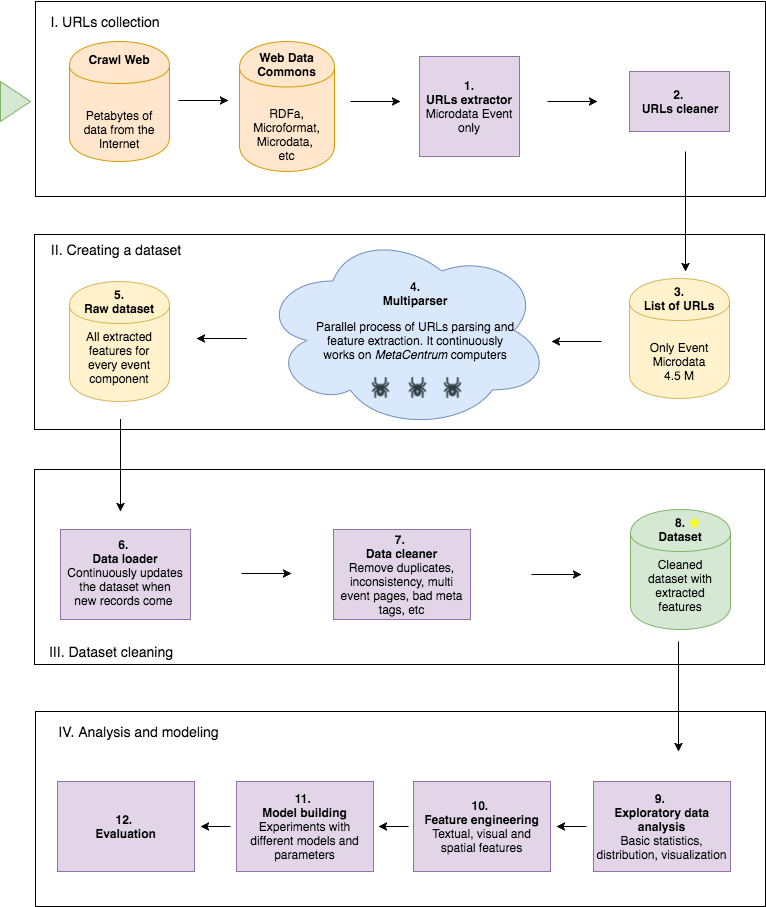
\includegraphics[width=1.0\textwidth]{figures04/Architecure}
\caption{The components of Sociopath event extraction system}
\label{fig:architecture}
\end{center}
\end{figure}

On the picture \nameref{fig:architecture} you see the detailed schema of the application. Below you will find the description of every component from this schema.\\

\textbf{Common Crawl} is a project which collects and maintain the most comprehensive public corpus of web crawl data. Common Crawl's web archive consists of more than 250 TiB of content from more than 3 billion webpages \cite{commoncrawl}. It completes the crawls every month, and the history is available for the last eight years. The corpus contains raw web page data, extracted meta-data, and text.

\textbf{Web Data Common (WDS)}\cite{webdatacommons} is built on Common Crawl. It extracts the structured data (RDFa, Microdata, Microformat, and Embedded JSON-LD) from the Common Crawl corpus quarterly and shares the dataset for public download to support researcher and companies. 

\textbf{1. URLs extractor}. This component takes as an input the data from WDC which is a huge text file which consists of N-Quad rows. An example of such format you will see in the section \nameref{sec:urlparse}. The goal of URLs extractor is collecting only URL addresses of those pages which contain the \textit{Event} Microdata semantic markup together with all its successor as \textit{SocialEvent}, \textit{SportsEvent}, etc.\\

\textbf{2. URLs cleaner}. This component ensures that all URLs exists, available, and have the correct structure. After we collected the URLs, we put them in the storage of URLs chunks. Every piece consists of 100 URLs with Event Microdata. We keep the data like this in the \textbf{3. List of URLs} component because it would be more convenient to process later.\\

\textbf{4. Multiparser} and \textbf{5. Raw dataset}. The Multiparser is the most time-consuming part of the workflow. It is a parallel program which runs several independent processes for crawling the URLs. Every crawler does three things: loading, feature extraction, and features writing. The raw dataset contains two types of records: features of the event components and features of the random elements of the page to collect negative examples too. We run the parser on MetaCentrum distributed computer system.\\

\textbf{6. Data loader} and \textbf{7. Data cleaner}. Data loader component loads the raw data from the MetaCentrum through the SSH connector.  Data cleaner executes extensive cleaning procedure such that the number of records has decreased ten times. We will discuss the cleaning procedure in chapter \nameref{chap:clean}.\\

\textbf{8. Final dataset.} The raw dataset contains event components and random elements together with associated web features and identifiers.\\

\textbf{9. Exploratory data analysis}. In this part, we visualized and learned every feature, its basic statistics, the form of distribution and its specificity. Also, we experiment with dimensionality reduction methods.  \\

\textbf{10. Feature engineering and selection}. On this stage, we made a feature engineering and created features that can be divided into three parts: spatial, textual and visual. Also, we run several Random Forests classifiers to reveal the importance of the features.\\

\textbf{11. Model building and 12. Evaluation} In this part we experimented with different classification models, optimized their parameters and compare results on previously unseen data. \\

\section{Tools}

Here is a list of the primary tools and frameworks which we used for building the Sociopath event extraction system. All used tools are free and open-source.\\

\noindent\textbf{Used programming languages:} \textit{Python} for all processing, parsing and data analysis procedures; \textit{JavaScript} for DOM manipulation inside the virtual browser.\\

\noindent\textbf{Python stack:} \textit{sklearn, pandas, numpy} libraries for data manipulation and model building; \textit{NLTK} toolkit for textual features engineering;  \textit{xgboost} framework for boosted trees algorithm; \textit{multiprocessing} library for parallel parsing process. \\

\noindent\textbf{Webpage crawling:} \textit{PhantomJS} virtual browser; \textit{urllib2, Scrapy} frameworks for retrieving data from a URL webpage with CSS and XPath selectors.\\

\noindent\textbf{Visualization:} \textit{Matplotlib, Seaborn and Bokeh} - Python libraries for dataset visualization, \textit{draw.io} - web service for creating diagrams. \\

\noindent\textbf{Computation:} \textit{Local computer} -- Mac OS, Processor 2,7GHz Intel Core i5, RAM 16 GB; \textit{Remote computation} -- \textit{MetaCentrum} virtual distributed computing infrastructure (free for CTU students).\\

\noindent\textbf{SSH connection:} \textit{Paramiko} for Python code, \textit{Cyberduck} and terminal for a desktop.\\

\noindent\textbf{IDE:} PyCharm IDE and Jupyter Notebook.\\

\section*{Conclusion of the chapter}
In this chapter, we presented the scheme of the Sociopath event extraction system, and briefly explained its main components. In the next sections, we will cover all parts of the system. Also, we provided the list of technologies and tools which we actively use during the work. 